%%%%%%%%%%%%%%%%%%%%%%%%%%%%%%%%%%%%%%%%%%%%%%%%%%%%%%%%%%%%%%%%%%%%%%%%%%%%%%%%
% Preámbulo                                                                    %
%%%%%%%%%%%%%%%%%%%%%%%%%%%%%%%%%%%%%%%%%%%%%%%%%%%%%%%%%%%%%%%%%%%%%%%%%%%%%%%%

\documentclass[11pt,a4paper,titlepage,oneside]{report}

%%% RELACIÓN DE VARIABLES A PERSONALIZAR %%%
%\def\lingua{gal}
\def\lingua{esp} % descomenta esta liña se redactarás a memoria en español
%\def\lingua{eng} % descomenta esta liña se redactarás a memoria en inglés
\def\nome{Ángel Barral de Jesús}                             % substitúe aquí o teu nome
\def\nomedirectorA{Carlos Vázquez Regueiro}              % substitúe aquí o nome de quen dirixe
\def\nomedirectorB{Juan Antonio Martín Pernas}             % duplica esta liña máis veces se o precisas, cambiando
                                                     % a letra final (A, B, C, D...): úsanse na portada.tex
\def\titulo{Desarrollo de una interfaz interactiva de navegación de registros históricos personalizados integrada con un sistema de asistencia en procesos de empresa} % substitúe aquí o título do teu TFG
%\def\titulacion{gced}                               % descomenta esta liña e comenta a seguinte se es estudante do GCED
\def\titulacion{gei}
%\def\mencion{COMPUTACIÓN}                           % descomenta a mención que che corresponda se es estudante do GEI
\def\mencion{ENXEÑARÍA DO SOFTWARE}
%\def\mencion{ENXEÑARÍA DE COMPUTADORES}
%\def\mencion{SISTEMAS DE INFORMACIÓN}
%\def\mencion{TECNOLOXÍAS DA INFORMACIÓN}

%\def\renomearcadros{si} % descomenta esta liña se redactas a memoria en español e prefires que
                         % os "cuadros" e o "índice de cuadros" se renomeen
                         % a "tablas" e "índice de tablas" respectivamente

\usepackage{estilo_tfg}

% Lista de paquetes potencialmente interesantes (uso baixo demanda)

% \usepackage{alltt}       % proporciona o entorno alltt, semellante a verbatim pero que respecta comandos
% \usepackage{enumitem}    % permite personalizar os entornos de lista
% \usepackage{eurofont}    % proporciona o comando \euro
% \usepackage{float}       % permite máis opcións para controlar obxectos flotantes (táboas, figuras)
% \usepackage{hhline}      % permite personalizar as liñas horizontais en arrays e táboas
  \usepackage{longtable}   % permite construir táboas que ocupan máis dunha páxina
% \usepackage{lscape}      % permite colocar partes do documento en orientación apaisada
% \usepackage{moreverb}    % permite personalizar o entorno verbatim
  \usepackage{multirow}    % permite crear celdas que ocupan varias filas da mesma táboa
% \usepackage{pdfpages}    % permite insertar ficheiros en PDF no documento
% \usepackage{rotating}    % permite diferentes tipos de rotacións para figuras e táboas
% \usepackage{subcaption}  % permite a inclusión de varias subfiguras nunha figura
% \usepackage{tabu}        % permite táboas flexibles
% \usepackage{tabularx}    % permite táboas con columnas de anchura determinada

%%%%%%%%%%%%%%%%%%%%%%%%%%%%%%%%%%%%%%%%%%%%%%%%%%%%%%%%%%%%%%%%%%%%%%%%%%%%%%%%
% Corpo                                                                        %
%%%%%%%%%%%%%%%%%%%%%%%%%%%%%%%%%%%%%%%%%%%%%%%%%%%%%%%%%%%%%%%%%%%%%%%%%%%%%%%%

\begin{document}

 %%%%%%%%%%%%%%%%%%%%%%%%%%%%%%%%%%%%%%%%
 % Preliminares do documento            %
 %%%%%%%%%%%%%%%%%%%%%%%%%%%%%%%%%%%%%%%%

 \begin{titlepage}
  
  \hspace*{128pt}
  \textcolor{udcpink}{{\fontencoding{T1}\fontfamily{phv}\selectfont Facultade de Informática}}\\[-32pt]

  \begin{center}
    
\includegraphics[scale=0.3]{imaxes/udc}\\[25pt]

    {\large TRABALLO FIN DE GRAO \\
            \nometitulacion \\
            \nomemencion } \\[10pt]

    \carimbo \\[25pt]

    \begin{huge}
      \begin{spacing}{1.3}
        \bfseries \titulo
      \end{spacing}
    \end{huge}
  \end{center}
  
  \vfill
  
  \begin{flushright}
    {\large
    \begin{tabular}{ll}
      {\bf Estudante:} & \nome \\
      {\bf Dirección:} & \nomedirectorA \\
                      & \nomedirectorB \\ % duplica esta liña máis veces se o precisas, cambiando
                                           % a letra final (A, B, C, D...); define eses nomes no memoria_tfg.tex
    \end{tabular}}
  \end{flushright}
  \rightline{A Coruña, \datasimple.}
\end{titlepage}

 \dedicatoria{Dedicatoria} % escribe neste comando o teu texto de dedicatoria
 \paxinaenbranco
 \begin{agradecementos}
 \blindtext                % substitúe este comando polo teu texto de agradecementos
 \end{agradecementos}
 %%%%%%%%%%%%%%%%%%%%%%%%%%%%%%%%%%%%%%%%%%%%%%%%%%%%%%%%%%%%%%%%%%%%%%%%%%%%%%%%

\pagestyle{empty}
\begin{abstract}

    Este proyecto consiste en la creación de una interfaz interactiva para generar informes de forma sencilla mediante expresiones de lenguaje natural que va 
    añadiendo el usuario. 

    Su objetivo principal es que, utilizando los datos recogidos anteriormente mediante SINVAD, esta interfaz nos permite manipularlos o consultarlos
    de tal forma que haciendo llamadas a su API, recupere los datos que el usuario esta buscando.

    Esto nos permitirá generar informes de cualquiera de los datos que este en el histórico. Para esto será necesario analizar estas expresiones naturales
    y procesar las palabras claves que se utilizarán para buscar los datos que necesatimos.

    La idea con esto, es que los usuario que vayan utilizar esta interfaz no pierdan parte importante de su trabajo en configurar el informe, sino que mediante 
    unas simples expresiones y con un diseño intuitivo con ejemplos para cualquiera persona ajena al mundo tecnologico, sea capaz
    de generar informes de forma sencilla. 


  \vspace*{50pt}
  \begin{segundoresumo}

    This project consists of creating an interactive interface to generate reports in a simple way using natural language expressions.

    Its main objective is that, using the data previously collected in SINVAD, this interface allows us to manipulate or consult them
    in such a way that by making calls to the SINVAD Rest API, the data that the user is looking for is recovered.

    This will allow us to generate reports of any of the data that is in the history. For this, it will be necessary to analyze these natural expressions
    and extract the key words that will be used to search for the data we need.

    The idea with this is that the users who are going to use this interface do not lose an important part of their work in configuring the report, but rather that through
    some simple expressions and with an intuitive design with examples for anyone outside the technological world, they will be able
    to generate reports in a simple way.

  \end{segundoresumo}
\vspace*{50pt}
\begin{multicols}{2}
\begin{description}
\item [\palabraschaveprincipal:] \mbox{} \\[-20pt]
  \blindlist{itemize}[7] % substitúe este comando por un itemize
                         % que relacione as palabras chave
                         % que mellor identifiquen o teu TFG
                         % no idioma principal da memoria (tipicamente: galego)
\end{description}
\begin{description}
\item [\palabraschavesecundaria:] \mbox{} \\[-20pt]
  \blindlist{itemize}[7] % substitúe este comando por un itemize
                         % que relacione as palabras chave
                         % que mellor identifiquen o teu TFG
                         % no idioma secundario da memoria (tipicamente: inglés)
\end{description}
\end{multicols}

\end{abstract}
\pagestyle{fancy}

%%%%%%%%%%%%%%%%%%%%%%%%%%%%%%%%%%%%%%%%%%%%%%%%%%%%%%%%%%%%%%%%%%%%%%%%%%%%%%%%


 \pagenumbering{roman}
 \setcounter{page}{1}
 \bstctlcite{IEEEexample:BSTcontrol}

 \tableofcontents
 \listoffigures
 \listoftables
 \clearpage
 
 \pagenumbering{arabic}
 \setcounter{page}{1}

 %%%%%%%%%%%%%%%%%%%%%%%%%%%%%%%%%%%%%%%%
 % Capítulos                            %
 %%%%%%%%%%%%%%%%%%%%%%%%%%%%%%%%%%%%%%%%

 \chapter{Introdución}
\label{chap:introducion}

\section{Contexto}

\lettrine Cualquier persona de una empresa pierde gran parte de su tiempo para ser capaz de acceder a la información 
que necesita para llevar su trabajo o en registrar nuevos datos en un sistema de información de una empresa. 

Para solucionar esto tenemos SINVAD, un sistema de compresión de lenguaje natural que es desarrollado por la empresa SREC Solutions. 
El objetivo es asistir al usuario para consultar información, registrar datos y supervisar información desde cualquier dispositivo con sus propias palabras, 
en múltiples idiomas y adaptado a los procesos de empresa.

Pero esto tiene una gran limitación, y es que el cliente debe construir sus propias aplicaciones para integrar la API REST de 
SINVAD para así poder generar informes a partir de los registros de los históricos del cliente.

Por tanto, el objetivo de este proyecto es generar una interfaz interactiva de navegación de históricos asociados que 
facilite la integración de la API de SINVAD y nos permita gestionar la generación, consulta, interacción, edición en tiempo real, 
descarga y generación de notificaciones en tiempo real de estos informes que se nombraron anteriormente.

Se busca que esta interfaz sea fácil de utilizar y intuitiva, para que cualquiera persona de cualquiera edad sepa utilizarla, 
y mediante unas pocas y sencillas acciones, sea capaz de generar informes sobre cualquiera de los datos que tienen el histórico.

\section{Objetivos}

En relación con lo anterior, a continuación se detallarán los objetivos que debería cumplir nuestra interfaz.

Esta interfaz debe estar disponible vía web y cualquier usuario que tenga acceso tiene que ser capaz de utilizarla de forma sencilla.
Para esto buscaremos que nuestra interfaz sea intuitiva y con esto nos referimos que cualquiera persona, con o sin conocimientos tecnologicos,
sea capaz mediante una serie sencilla de pasos, sacar los informes que a ellos le interesen.

Dentro de esta interfaz, el usuario podrá hacer los siguientes pasos:

- \textbf{Título del informe:} El usuario, antes de empezar a configurar la información que quiere que aparezca en el informe, necesitará indicar el propósito por el cuál se crea, y
esto se indicará mediante el título.

- \textbf{Periocidad del informe:} El usuario podrá indicar la periocidad con la que quiere generar el informe, ya que estos, se generarán automáticamente cada x tiempo.

- \textbf{Número de columnas:} El usuario podrá elegir el número de columnas que aparezcan en su informe y el contenido de cada una de ellas. Si alguna de estas, no muestra
el dato correcto, se podrá editar antes de generar el informe.

- \textbf{Contenido del informe: } Al seleccionar el número de columnas, aparte del título de estas, será necesario el dato a buscar mediante una expresión de lenguaje natural, y 
esto será lo que el usuario le pasará a nuestro LLM para que lo procese.

Para cumplir todos estos pasos, la interfaz los contendrá de forma sencilla y intuitiva como se mostrará mas adelante en este documento, para facilitar al usuario
este proceso lo máximo posible.


% \chapter{Contido demostrativo}
\label{chap:demo}

\lettrine{E}{ntre} a introdución e as conclusións, o documento conterá
tantos capítulos como sexa preciso, sempre con coidado de non rebasar
o límite de 80 páxinas fixado polo regulamento de TFGs.

Empregaremos éste de xeito demostrativo, para ilustrar o uso de
elementos habituais que poidan ser de utilidade\footnote{Por exemplo,
  isto é unha nota a pé de páxina.}.

\section{Inclusión de imaxes}

Se precisamos imaxes no noso documento, incluirémolas do xeito que se
indica na figura~\ref{fig:exemplo} (páxina~\pageref{fig:exemplo}). Se
o facemos así, \LaTeX ubicará cada imaxe no mellor lugar posible,
lugar que pode variar a medida que o documento vaia crecendo coa
inclusión de máis texto e outros elementos (máis imaxes, táboas,
etc.).

\begin{figure}[hp!]
  \centering
  
\includegraphics[width=0.75\textwidth]{imaxes/udc.png}
  \caption{Pé de imaxe descritivo}
  \label{fig:exemplo}
\end{figure}

Recoméndase almacenar os ficheiros gráficos no directorio
\texttt{imaxes}.

\subsection{Inclusión de varias sub-imaxes}

Se precisamos inserir imaxes relacionadas, pode ser apropiado
incluílas como sub-figuras, do xeito que se pode apreciar na
figura~\ref{fig:exemplo-subfiguras} (páxina~\pageref{fig:exemplo-subfiguras})
coas imaxes~\ref{fig:subfigura-rotada} e~\ref{fig:subfigura-deformada}.
Como se pode ver nos exemplos desta sección, sempre é recomendable
referirse ás imaxes (ou táboas e outros elementos \emph{flotantes},
que se demostrarán nas seccións seguintes deste capítulo demostrativo)
pola súa referencia, xa que dese xeito non dependemos de onde
queden ubicados os elementos en cuestión.

\begin{figure}[hp!]
  \centering
  \begin{subfigure}[c]{0.3\textwidth}
    
\includegraphics[angle=45,width=\textwidth]{imaxes/udc.png}
    \caption{Pé de subimaxe rotada}
    \label{fig:subfigura-rotada}
  \end{subfigure}
  \hspace{0.1\textwidth}
  \begin{subfigure}[c]{0.3\textwidth}
    
\includegraphics[width=\textwidth,height=3cm]{imaxes/udc.png}
    \caption{Pé de subimaxe deformada}
    \label{fig:subfigura-deformada}
  \end{subfigure}
  \caption{Pé de imaxe xeral}
  \label{fig:exemplo-subfiguras}
\end{figure}

\section{Inclusión de táboas}

Se precisamos táboas no noso documento, incluirémolas do xeito que se
indica na táboa~\ref{tab:exemplo} (páxina~\pageref{tab:exemplo}). Se
o facemos así, \LaTeX ubicará cada táboa no mellor lugar posible,
lugar que pode variar a medida que o documento vaia crecendo coa
inclusión de máis texto e outros elementos (máis imaxes, táboas,
etc.).

\begin{table}[hp!]
  \centering
  \rowcolors{2}{white}{udcgray!25}
  \begin{tabular}{c|c}
  \rowcolor{udcpink!25}
  \textbf{Título de columna} & \textbf{Outro título de columna} \\\hline
  \textit{Título de fila} & Contido da cela \\
  \textit{Título de fila} & Contido da cela \\
  \textit{Título de fila} & Contido da cela \\
  \textit{Título de fila} & Contido da cela \\
  \textit{Título de fila} & Contido da cela \\
  \textit{Título de fila} & Contido da cela \\
  \end{tabular}
  \caption{Pé de táboa descritivo}
  \label{tab:exemplo}
\end{table}

\subsection{Inclusión de táboas longas}

Para táboas longas que ocupan varias páxinas, como é o caso da \ref{tab:longa}
(páxina~\pageref{tab:longa}), recoméndase o uso do paquete \texttt{lontable},
incluído xa entre os paquetes recomendados no ficheiro raíz do proxecto
(\verb+memoria_tfg.tex+).

{\rowcolors{2}{white}{udcgray!25}
\begin{longtable}{l|r|c}
  \caption{Pé descritivo dunha táboa longa}
  \label{tab:longa} \\

  \rowcolor{udcpink!25}
  \textbf{Primeira columna} & \textbf{Segunda columna} & \textbf{Terceira columna} \\\hline
  \endfirsthead

  \multicolumn{3}{c}{\tablename\ \thetable{} -- {\small \textit{(vén da páxina anterior)}}} \\
  \rowcolor{udcpink!25}
  \textbf{Primeira columna} & \textbf{Segunda columna} & \textbf{Terceira columna} \\\hline
  \endhead

  \multicolumn{3}{c}{\dotfill{\small \textit{(continúa na páxina seguinte)}}\dotfill} \\
  \endfoot

  \endlastfoot

  Texto de exemplo & abcdef ghjijklmn & 123.456778 \\
  Texto de exemplo & abcdef ghjijklmn & 123.456778 \\
  Texto de exemplo & abcdef ghjijklmn & 123.456778 \\
  Texto de exemplo & abcdef ghjijklmn & 123.456778 \\
  Texto de exemplo & abcdef ghjijklmn & 123.456778 \\
  Texto de exemplo & abcdef ghjijklmn & 123.456778 \\
  Texto de exemplo & abcdef ghjijklmn & 123.456778 \\
  Texto de exemplo & abcdef ghjijklmn & 123.456778 \\
  Texto de exemplo & abcdef ghjijklmn & 123.456778 \\
  Texto de exemplo & abcdef ghjijklmn & 123.456778 \\
  Texto de exemplo & abcdef ghjijklmn & 123.456778 \\
  Texto de exemplo & abcdef ghjijklmn & 123.456778 \\
  Texto de exemplo & abcdef ghjijklmn & 123.456778 \\
  Texto de exemplo & abcdef ghjijklmn & 123.456778 \\
  Texto de exemplo & abcdef ghjijklmn & 123.456778 \\
  Texto de exemplo & abcdef ghjijklmn & 123.456778 \\
  Texto de exemplo & abcdef ghjijklmn & 123.456778 \\
  Texto de exemplo & abcdef ghjijklmn & 123.456778 \\
  Texto de exemplo & abcdef ghjijklmn & 123.456778 \\
  Texto de exemplo & abcdef ghjijklmn & 123.456778 \\
  Texto de exemplo & abcdef ghjijklmn & 123.456778 \\
  Texto de exemplo & abcdef ghjijklmn & 123.456778 \\
  Texto de exemplo & abcdef ghjijklmn & 123.456778 \\
  Texto de exemplo & abcdef ghjijklmn & 123.456778 \\
  Texto de exemplo & abcdef ghjijklmn & 123.456778 \\
  Texto de exemplo & abcdef ghjijklmn & 123.456778 \\
  Texto de exemplo & abcdef ghjijklmn & 123.456778 \\
  Texto de exemplo & abcdef ghjijklmn & 123.456778 \\
  Texto de exemplo & abcdef ghjijklmn & 123.456778 \\
  Texto de exemplo & abcdef ghjijklmn & 123.456778 \\
  Texto de exemplo & abcdef ghjijklmn & 123.456778 \\
  Texto de exemplo & abcdef ghjijklmn & 123.456778 \\
  Texto de exemplo & abcdef ghjijklmn & 123.456778 \\
  Texto de exemplo & abcdef ghjijklmn & 123.456778 \\
  Texto de exemplo & abcdef ghjijklmn & 123.456778 \\
  Texto de exemplo & abcdef ghjijklmn & 123.456778 \\
  Texto de exemplo & abcdef ghjijklmn & 123.456778 \\

\end{longtable}
} % alcance do rowcolors que precede á táboa longa


\subsection{Inclusión de táboas con celas que ocupan varias columnas ou filas}

En ocasións pode resultar de interese incluír nunha táboa unha cela que se estenda
a través de varias columnas, como ocorre na táboa~\ref{tab:exemplocolumnas}
(páxina~\pageref{tab:exemplocolumnas}).

\begin{table}[hp!]
  \centering
  \rowcolors{2}{white}{udcgray!25}
  \begin{tabular}{c|c|c}
  \rowcolor{udcpink!25}
  \multicolumn{3}{c}{\textbf{Cela en varias columnas}} \\\hline
  \rowcolor{udcpink!25}
  \textbf{Título de columna} & \textbf{Outro título de columna} & \textbf{Outro título máis} \\\hline
  \textit{Título de fila}    & Contido da cela                  & Contido da cela \\
  \textit{Título de fila}    & Contido da cela                  & Contido da cela \\
  \textit{Título de fila}    & \multicolumn{2}{c}{Contido da cela múltiple} \\
  \textit{Título de fila}    & Contido da cela                  & Contido da cela \\
  \end{tabular}
  \caption{Pé de táboa descritivo (táboa con celas que ocupan varias columnas)}
  \label{tab:exemplocolumnas}
\end{table}

Tamén pode resultar necesario facer o propio mais en varias filas da mesma columna,
como ocorre na táboa~\ref{tab:exemplofilas} (páxina~\pageref{tab:exemplofilas}).
Para isto é preciso o paquete \texttt{multirow}, incluído entre os recomendados no
ficheiro raíz do proxecto (\verb+memoria_tfg.tex+).

O uso de celas multifila requerirá do xuste da coloración das filas, a fin de manter
a coherencia entre o contido e o continente. Así, no canto de usar un único comando
\verb+rowcolors+ para indicar a alternancia en toda a táboa, usaremos o comando
\verb+rowcolor+ antes dunha fila que queiramos colorear, e o comando \verb+cellcolor+
dentro dunha cela que queiramos colorear.

\begin{table}[hp!]
  \centering
  \begin{tabular}{c|c}
  \rowcolor{udcpink!25}
  \textbf{Título de columna} & \textbf{Outro título de columna} \\\hline
  \multirow{2}{*}{\textit{Título de fila}} & \cellcolor{udcgray!25} Contido da cela \\
                                           & Contido da cela \\
  \rowcolor{udcgray!25}
  \textit{Título de fila}                  & Contido da cela \\
  \multirow{3}{*}{\textit{Título de fila}} & Contido da cela \\
                                           & \cellcolor{udcgray!25} Contido da cela \\
                                           & Contido da cela \\
  \rowcolor{udcgray!25}
  \textit{Título de fila}                  & Contido da cela \\
  \end{tabular}
  \caption{Pé de táboa descritivo (táboa con celas que ocupan varias filas)}
  \label{tab:exemplofilas}
\end{table}

Por suposto, pódense combinar nunha mesma táboa os dous tipos de celas (as que se 
estenden máis dunha fila e máis dunha columna), como na táboa~\ref{tab:exemplofilasecolumnas}
(páxina~\pageref{tab:exemplofilasecolumnas}).

\begin{table}[hp!]
  \centering
  \begin{tabular}{c|c|c}
  \rowcolor{udcpink!25}
  \multicolumn{3}{c}{\textbf{Cela en varias columnas}} \\\hline
  \rowcolor{udcpink!25}
  \textbf{Título de columna}               & \textbf{Outro título de columna}             & \textbf{Outro título máis} \\\hline
  \multirow{2}{*}{\textit{Título de fila}} & \cellcolor{udcgray!25} Contido da cela       & \cellcolor{udcgray!25} Contido da cela \\
                                           & Contido da cela                              & Contido da cela \\
  \rowcolor{udcgray!25}
  \textit{Título de fila}                  & \multicolumn{2}{c}{Contido da cela múltiple} \\
  \multirow{3}{*}{\textit{Título de fila}} & Contido da cela                              & Contido da cela \\
                                           & \multicolumn{2}{c}{\cellcolor{udcgray!25} Contido da cela múltiple} \\
                                           & \multicolumn{2}{c}{Contido da cela múltiple} \\
  \rowcolor{udcgray!25}
  \textit{Título de fila}                  & Contido da cela                              & Contido da cela \\
  \end{tabular}
  \caption{Pé de táboa descritivo (táboa con celas que ocupan varias columnas)}
  \label{tab:exemplofilasecolumnas}
\end{table}

\section{Inclusión de código fonte}

Se precisamos incluír fragmentos de código fonte, podemos facelo, por exemplo, da
seguinte maneira:

\begin{lstlisting}[language=C]
#include <stdio.h>
#define N 10

int main()
{
  int i;

  // Isto é un comentario
  puts("Ola, mundo!");

  for (i = 0; i < N; i++)
  {
    puts("LaTeX é a ferramenta de edición ideal para profesionais da informática!");
  }

  return 0;
}
\end{lstlisting}

\section{Uso da relación de acrónimos e do glosario}

Os acrónimos edítanse no ficheiro \texttt{bibliografia/acronimos.tex}
e úsanse empregando a orde \texttt{acrlong} para obter o termo
completo (deste xeito: \acrlong{erlang}), a orde \texttt{acrshort}
para obter o acrónimo (deste xeito: \acrshort{erlang}). A primeira vez
que usamos un termo con acrónimo no documento é recomendable usar orde
\texttt{acrfull} (que produce ambas versións á vez:
\acrfull{erlang}). Os acrónimos que non se usan no documento, non
aparecen na relación que se xerar na versión PDF.

Pola súa banda, os termos do glosario edítanse no ficheiro
\texttt{bibliografia/glo\-sa\-rio.tex} e úsanse empregando a orde
\texttt{gls} (deste xeito, \gls{bytecode}) ou \texttt{Gls} (deste
xeito, \Gls{bytecode}). Ao igual que os acrónimos, os termos que non
se usan no documento, non aparecen na relación que se xera na versión
PDF.

 \include{contido/metodología}
 \chapter{Desarrollo}
\label{chap:Desarrollo}

\section{1º Iteración: Diseño de la interfaz.}

Lo primero era tener claro cuál sería el diseño más correcto de nuestra interfaz para que así fuera intuitivo y fácil de utilizar para el cliente. Contamos con que este vaya ser la persona más alejada de la tecnología posible y por tanto la interfaz sea intuitiva y fácil de utilizar. Se propusieron 3 opciones para realizar nuestro diseño:

\subsection{1º Opción}

En esta primera opción, se propuso una tabla donde el usuario indica en cada columna el nombre de datos que quiere y mediante un formulario con una ayuda de un LLM recupera los datos del histórico de la empresa.

\begin{figure}[hp!]
    \centering
    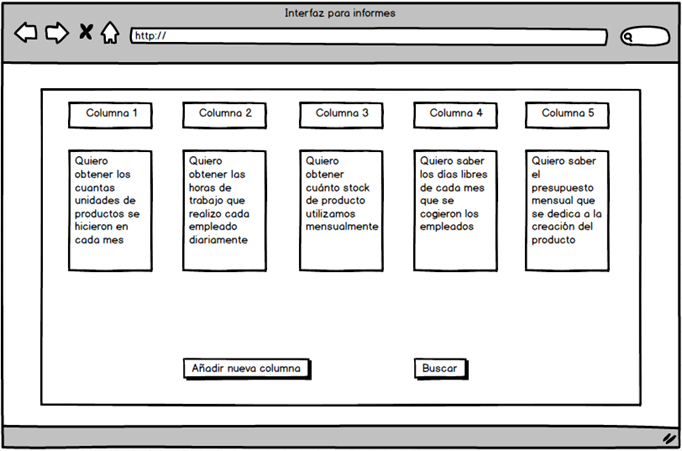
\includegraphics[width=0.75\textwidth]{imaxes/iteracion1.1.png}
    \caption{Primera opción: Tabla con datos para recuperar}
    \label{fig:iteracion1.1}
\end{figure}

El usuario podría introducir las columnas que quisiera e indicaría el nombre del dato que va a recuperar mediante el nombre de la columna. Con la ayuda de un formulario donde indicamos los datos que queremos recuperar y procesando esta información mediante un LLM, se recuperan estos datos del histórico.

\begin{figure}[hp!]
    \centering
    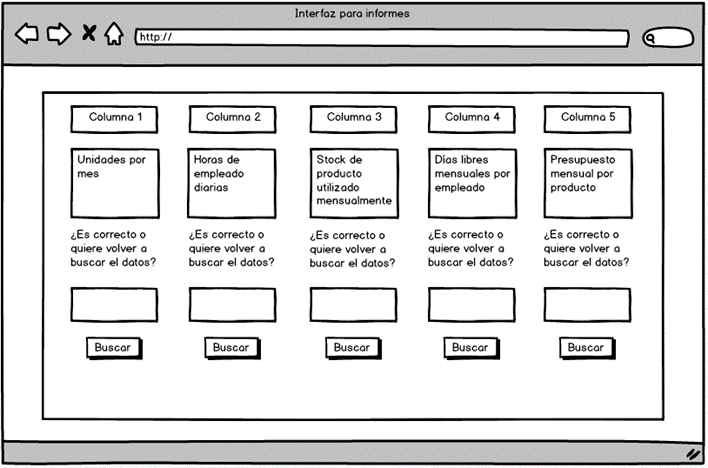
\includegraphics[width=0.75\textwidth]{imaxes/iteracion1.2.png}
    \caption{Primera opción: Tabla con datos recuperados y/o posibles modificaciones}
    \label{fig:iteracion1.2}
\end{figure}

Después de hacer la búsqueda con la ayuda del LLM, se mostrarán los datos que se recuperan de cada columna y tendrá la opción de editar alguno de estos datos sino es el que le interesa al cliente
  
Es una solución que permite guiar al usuario paso a paso para seleccionar los datos que quiere en su informe, pero tiene un gran problema, y es que, si añadimos muchas columnas, la interfaz se volverá muy compleja, ya que habría demasiada información y podría volverse muy confuso.

\subsection{2º Opción}

Esta segunda solución se basaría en un selector con los datos queremos ver, los seleccionamos e iremos avanzando progresivamente con más selectores hasta tener el dato concreto.

Primero de todo, el usuario selecciona los datos sobre las tablas que le interesa.

\begin{figure}[hp!]
    \centering
    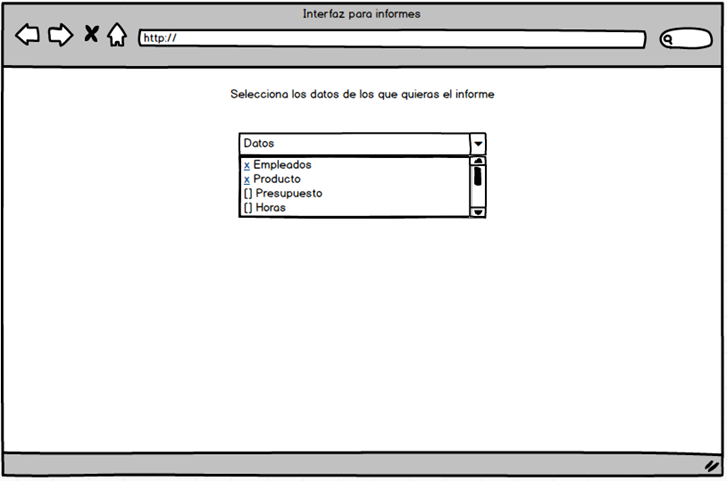
\includegraphics[width=0.75\textwidth]{imaxes/iteracion1.3.png}
    \caption{Segunda opción: Selector con primeras opciones}
    \label{fig:iteracion1.3}
\end{figure}

Después, se irán mostrando las distintas opciones de cada dato seleccionado e ir avanzando progresivamente mediante selectores.

\begin{figure}[hp!]
    \centering
    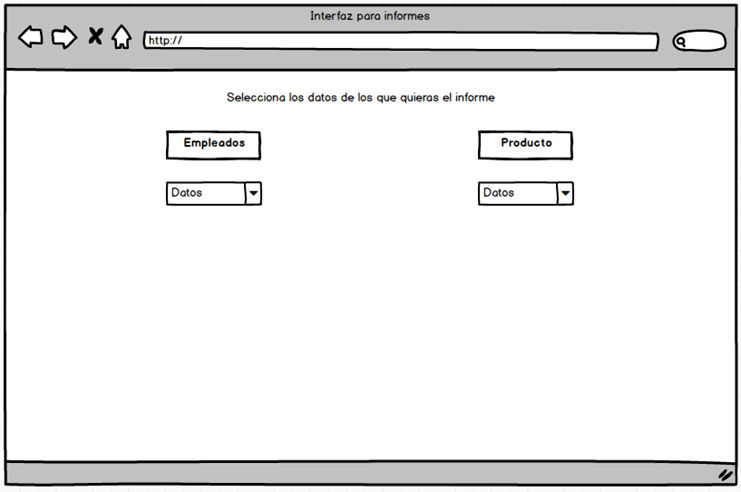
\includegraphics[width=0.75\textwidth]{imaxes/iteracion1.4.png}
    \caption{Segunda opción: Selector las siguientes opciones para acotar nuestro dato}
    \label{fig:iteracion1.4}
\end{figure}

En esta solución, los usuarios pueden ir seleccionando de manera progresiva lo que quieren en su informe, lo que puede ser bastante intuitivo para obtener los datos que queremos finalmente, pero tiene el mismo problema que la anterior, al seleccionar muchos datos, la interfaz se puede volver bastante engorrosa. También limita a la hora de crear informes complejos, ya que se necesitan muchos pasos para crearlos y puede ser una gran pérdida de tiempo para el cliente.

\subsection{3º Opción}

La tercera solución es un pront donde el usuario interactuara con un LLM viendo en un json o una tabla los datos que van ofreciendo y seleccionando los datos que más nos interesen mediante inputs.

\begin{figure}[hp!]
    \centering
    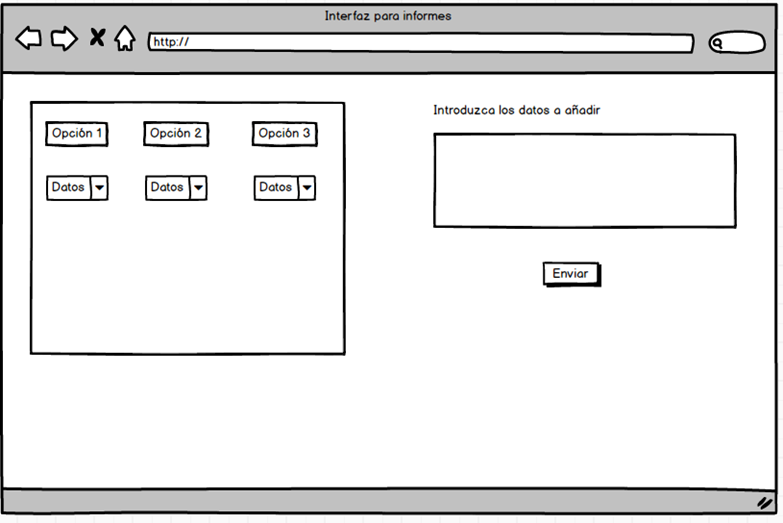
\includegraphics[width=0.75\textwidth]{imaxes/iteracion1.5.png}
    \caption{Tercera opción: Prompt con datos a añadir}
    \label{fig:iteracion1.5}
\end{figure}

El usuario introducirá los datos que le interese en el input y se irán mostrando las distintas opciones de datos para los elementos del informe generar.

Esta es una opción bastante buena para la generación de informes complejos, ya que con la ayuda del LLM puede ayudarnos a buscar lo que encontramos de forma correcto, pero esto se puede convertir en una contra también, ya que en el caso contrario podría ser que el LLM no entienda claramente lo que se quiere buscar y esto puede ser un problema para un usuario no familiarizado con la interfaz.

\subsection{Conclusión}

De estas 3 opciones, después de estudiar sus pros y contras, se concluyo que la mejor opción sería una mezcla de las 3 de esta forma.

Primero, el usuario seleccionará los datos de los que le interese generar el informe sin sus opciones.

\begin{figure}[hp!]
    \centering
    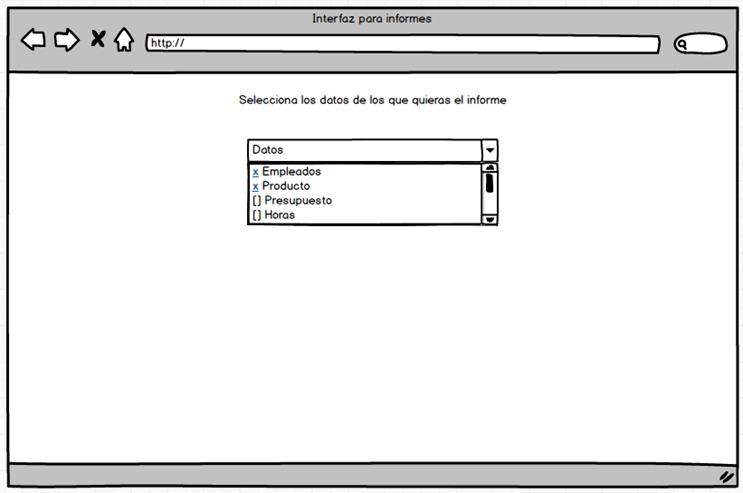
\includegraphics[width=0.75\textwidth]{imaxes/iteracion1.6.png}
    \caption{Conclusión: Seleccionamos los datos que nos interensan}
    \label{fig:iteracion1.6}
\end{figure}

Con los datos seleccionados, se nos mostrará una tablita donde con esos datos y un pront, el usuario indicará las opciones que quiere de cada dato recogiendo esa información con un LLM para posteriormente mostrarlo en la tabla.


\begin{figure}[hp!]
    \centering
    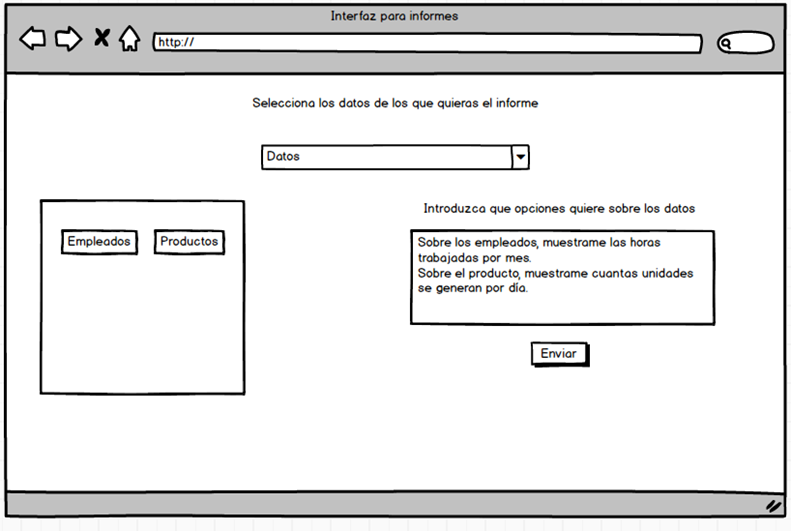
\includegraphics[width=0.75\textwidth]{imaxes/iteracion1.7.png}
    \caption{Conclusión: Tabla con los datos seleccionados y prompt para buscar}
    \label{fig:iteracion1.7}
\end{figure}

Cuando el LLM procesé la información, mostrará un selector desplegable donde se puede seleccionar la opción o las opciones que el usuario consideré opinión según lo introducido en el pront y su criterio.

\begin{figure}[hp!]
    \centering
    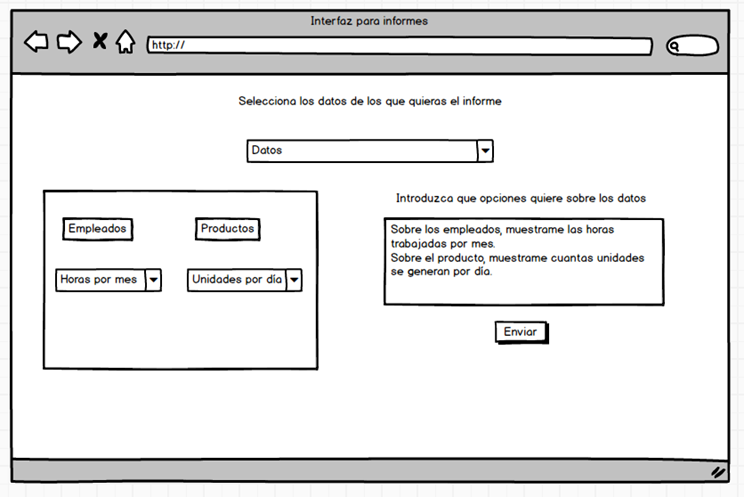
\includegraphics[width=0.75\textwidth]{imaxes/iteracion1.8.png}
    \caption{Conclusión: Tabla con los datos seleccionados y las opciones buscadas anteriormente}
    \label{fig:iteracion1.8}
\end{figure}
  
Esta es la mejor opción mezclando las 3 anteriores, ya que el usuario puede comenzar con una serie de columnas claras e ir modificándolas o no según su criterio. Con la ayuda del LLM, este nos muestra las opciones más acordes a nuestra búsqueda y ayudando así a no tener que navegar mediante selectores, lo cuál es mucho más engorroso para un usuario sin experiencia.
  
\section{2º Iteración: Nueva propuesta de diseño de la interfaz.}

Una vez comentandas las ideas anteriores junta UX, y tras refinarlas, se llego a una conclusión conjunta para como se quiere que sea esta interfaz.

En esta nueva pantalla, se nos mostrará diferentes opciones para configurar nuestro informe. Se podrá seleccionar la periodicidad con la que se generé (la idea de esta interfaz es que se generé cada x tiempo el informe una vez configurado), pudiendo seleccionar las unidades de tiempo y el período en el que se van a generar. Podemos ir añadiendo las columnas que creamos oportunas que aparezcan en él y en ellas indicar tanto el nombre como el dato que queremos buscar. 

\begin{figure}[hp!]
    \centering
    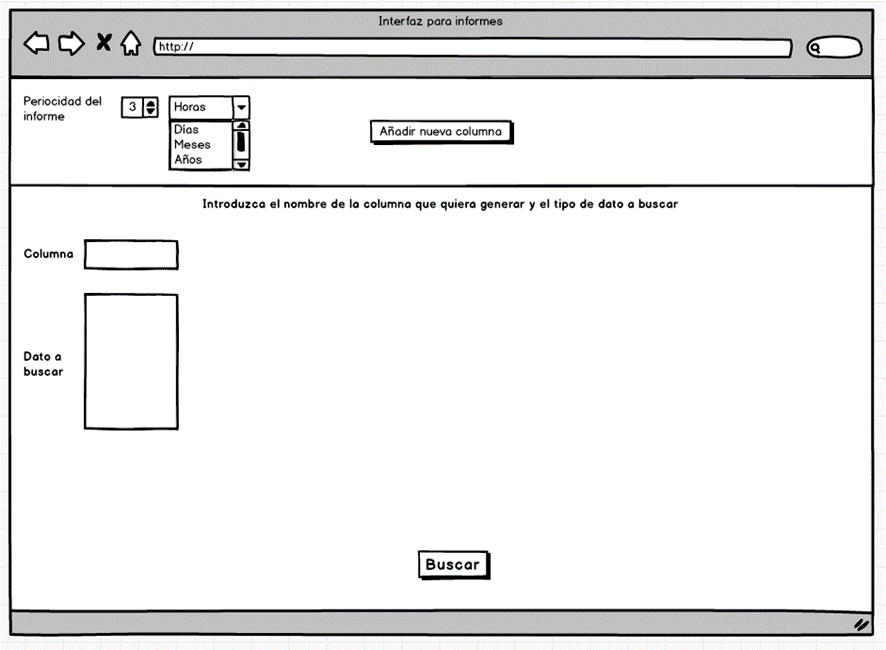
\includegraphics[width=0.75\textwidth]{imaxes/iteracion2.1.png}
    \caption{2º Iteración: Nueva interfaz}
    \label{fig:iteracion2.1}
\end{figure}

Una vez que introduzcamos la información que queremos, con la ayuda de un LLM, buscará está en nuestro histórico, para así mostrarle posteriormente los datos que busca el cliente.

\begin{figure}[hp!]
    \centering
    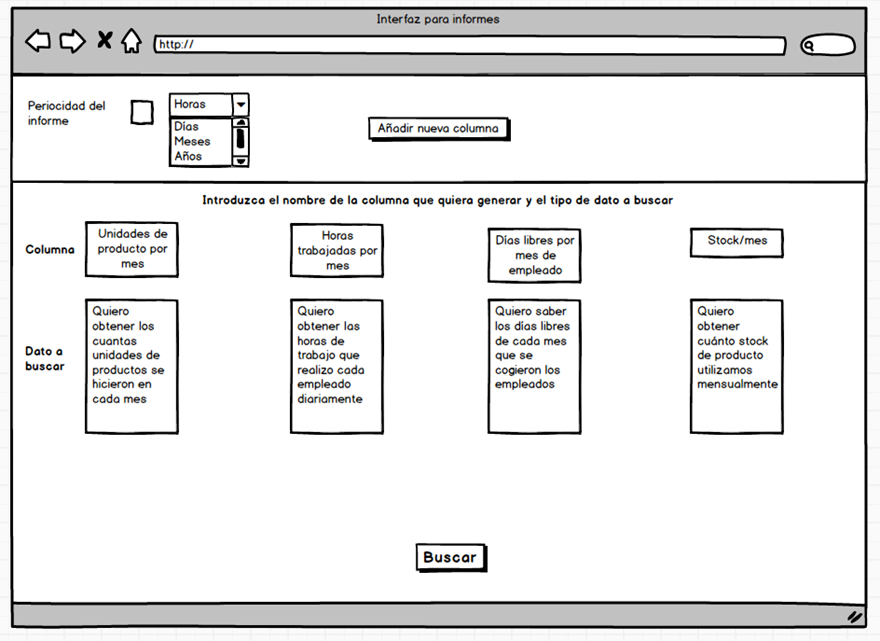
\includegraphics[width=0.75\textwidth]{imaxes/iteracion2.2.png}
    \caption{2º Iteración: Introducir columnas y datos para la busqueda}
    \label{fig:iteracion2.2}
\end{figure}

Si alguno de los datos que aparecen no nos encaja con lo que buscamos, podremos seleccionar mediante un desplegable la columna del informe que queremos cambiar y con la ayuda de un prompt, introduciremos los cambios que consideraremos oportunos.

Tendremos también una serie de palabras clave sugeridas para que así esta sea más fácil y nos facilite a la hora de generar el informe.

\begin{figure}[hp!]
    \centering
    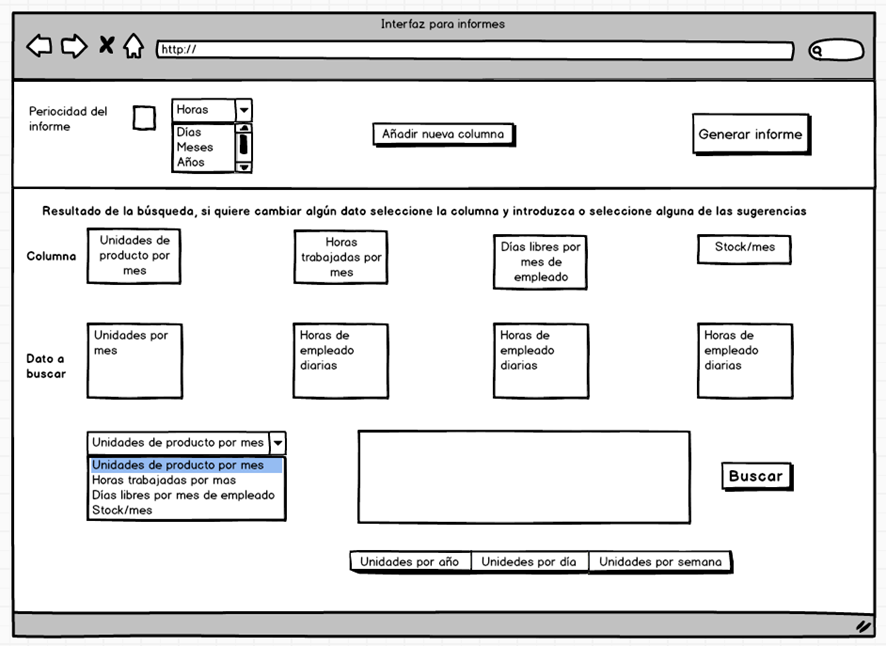
\includegraphics[width=0.75\textwidth]{imaxes/iteracion2.3.png}
    \caption{2º Iteración: Resultados de la búsqueda}
    \label{fig:iteracion2.3}
\end{figure}

\section{3º Iteración: Consolidación de la nueva propuesta.}

Se volvió a comentar la nueva propuesta con UX y se tomaron algunas decisiones de diseño para la interfaz. Primero de todo y más importante, habría que definir la finalidad de ese informe y esto se haría a través del título.

Se añadirá un título que describirá el propósito del informe. Para que sea más fácil para el usuario la configuración de este, se mostrará una serie de ejemplos donde el usuario podrá ver los diferentes pasos que debe seguir para generar el informe.

\begin{figure}[hp!]
    \centering
    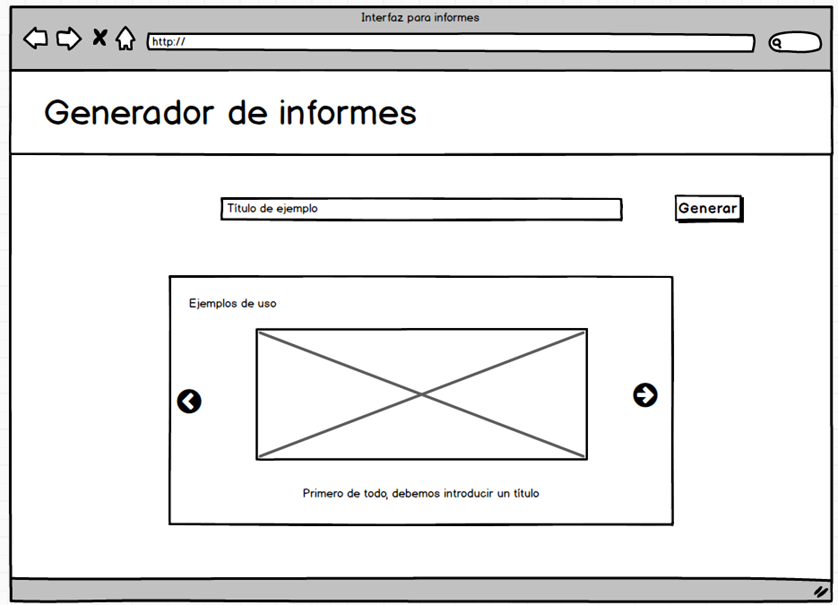
\includegraphics[width=0.75\textwidth]{imaxes/iteracion3.1.png}
    \caption{3º Iteración: Pantalla principal}
    \label{fig:iteracion3.1}
\end{figure}

Una vez añadido el título, deberíamos configurar el informe. Para esto seleccionaremos la periodicidad con la que se genera y el nombre de la columna más el dato que queremos añadir a nuestro informe, como se comentara en un principio. Si necesitamos añadir más datos a nuestro informe, añadiríamos una nueva columna a nuestra tabla.

\begin{figure}[hp!]
    \centering
    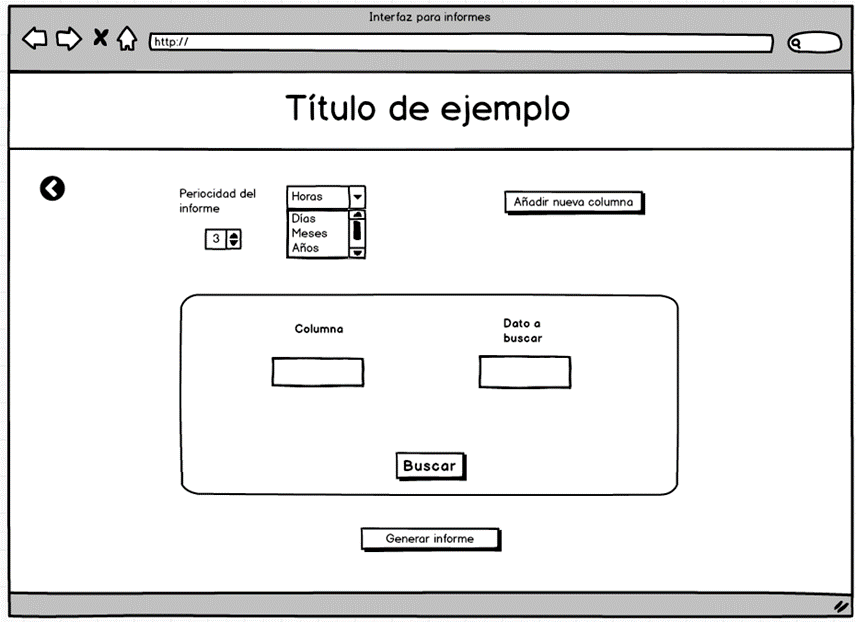
\includegraphics[width=0.75\textwidth]{imaxes/iteracion3.2.png}
    \caption{3º Iteración: Configurador de informe}
    \label{fig:iteracion3.2}
\end{figure}

En este caso, añadimos 2 columnas con los datos oportunos para buscarlos.

\begin{figure}[hp!]
    \centering
    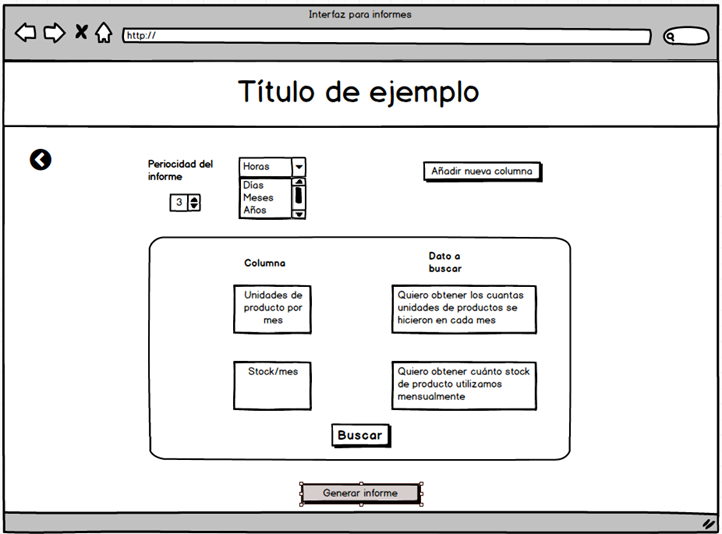
\includegraphics[width=0.75\textwidth]{imaxes/iteracion3.3.png}
    \caption{3º Iteración: Introducir datos de ejemplo para buscar}
    \label{fig:iteracion3.3}
\end{figure}

A la hora de buscar estos datos, nos mostraría las opciones que al LLM le pareció más oportuno según nuestros datos registrados en el histórico. Podemos seleccionar las distintas columnas de nuestro informe y mediante un prompt con algunas opciones sugeridas, poder refinar nuestra búsqueda para que nos muestre el dato de forma correcta

\begin{figure}[hp!]
    \centering
    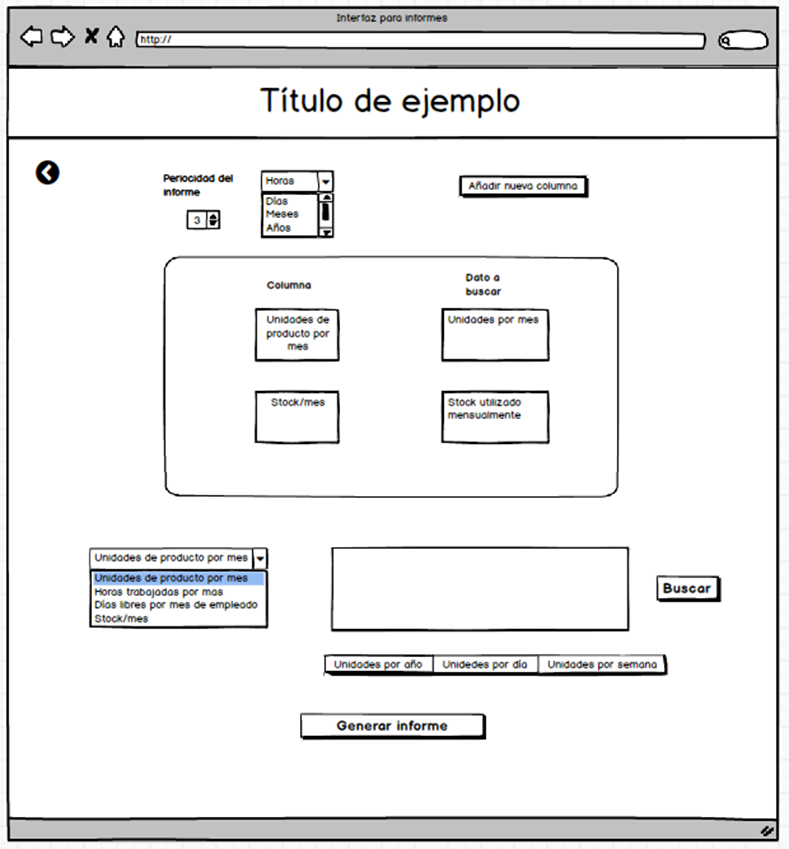
\includegraphics[width=0.75\textwidth]{imaxes/iteracion3.4.png}
    \caption{3º Iteración: Resultados de la búsqueda}
    \label{fig:iteracion3.4}
\end{figure}

Si tenemos claro que los datos son correctos, podemos generar nuestro informe, que quedara configurado para generarse periódicamente según el tiempo que le habremos indicado.
 \chapter{Fundamentos tecnologícos}
\label{chap:Fundamentos tecnologícos}

\section{Vue}

Vue es un framework de JavaScript que permite crear potentes y versátiles interfaces de usuario. Una de las grandes ventajas que tiene vue es que combina HTML, CSS y JavaScript en un mismo fichero, permitiéndonos tener más ordenado y localizable nuestro código. 

Este framework nos permite crear componente que después van poder ser reutlizados por otros componentes, lo que nos va dar una gran ventaja a la hora de ahorrar tiempo y costes en el proyecto.
Cada vez que hagamos un cambio en alguno de nuestro componente, este se actualiza automáticamente en la interfaz gracias a su propiedad reactiva.

Incluye algunas herramientas, como Vue Router, para gestionar el enrutamiento de las páginas que lo utilizaremos en el proyecto para nuestra interfaz.

Respecto a otros frameworks como Angular o React, vue nos proporcionan una serie de ventajas:

• Curva de aprendizaje suave: Es simple y fácil de aprender. Contiene bastante documentación clara, lo que permite desarrollar código de forma rápida.

• Flexibilidad respecto a frameworks como Angular, Vue permite al desarrollador elegir y configurar las partes que este considere oportunas únicamente.

• Tamaño ligero: Comparado con los otros frameworks, Vue.js es relativamente pequeño, lo que puede resultar de gran ayuda a la hora de tiempos de carga y rendimiento.

• Es muy parecido a HTML, por lo que la sintaxis es muy fácil de entender si ya trabajaste anteriormente con este. 


Utilizaremos este framework junta a Tailwindcss para el desarrollo de nuestra interfaz.

\section{TailwindCSS}

Tailwindcss es un framework de CSS que nos permite componer estilos de manera mucho más sencilla. Nos permite relacionar y crear clases css para utilizar en nuestros elementos HTML fácilmente.
	
A diferencia de Bootstrap o foundation, tailwind lo que nos proporcionan son conjunto de clases css de bajo nivel que son fácilmente combinables para así crear diseños sin la necesidad de escribir CSS personalizado.
	
Gracias a esta característica, nos proporciona un desarrollo de código más rápido al eliminar la necesidad de escribir todo el CSS personalizado para cada componente. 
	
Gracias al tener una clases de utilidad comunes, esto nos permite que el diseño en nuestra aplicación sea fácilmente mantenible y no preocuparnos de tener conflictos con los css.
	
Una clave en todo esto es que Tailwind no impone estilos predeterminados ni componentes específicos, lo que nos da una gran libertad a la hora de crear los diseños.
	
Por eso se eligio Tailwind, por su gran facilidad, flexibilidad y personalización a la hora de crear nuestro proyecto. 

\section{Shadcn-Vue}

Shadcn es una biblioteca de componentes que permite una fácil personalización de estos y de su estilo. Esto nos permite construir nuestra aplicación de forma eficiente y manejable, al utilizar componentes reutilizables.
	
La versión que utilizaremos en el proyecto es shadcn junto a vue o shadcn-vue, que permite una mayor facilidad a la hora de incluir los componentes, ya que estos están creados en vue.js.

Esto también nos permite que a la hora de añadir un componente, este se actualice automáticamente en la interfaz y si hacemos algún cambio en él, también se añada de forma correcta. 

\section{Visual Studio Code}

Visual Studio Code es un editor de código fuente desarrollado por Microsoft. Es conocido por ser ligero, rápido y extensible. Es gratuíto y de código abierto, lo que nos permite tener un gran variedad de extensiones para añadir a nuestro código.
	
Gracias a su gran variedad de lenguajes soportados, se eligió este ide ya que soporta Vue.js, por lo que es perfecto para desarrollar nuestra interfaz. También se eligió porque nos permite una serie de característica como son:
	
• Es ligero y rápido, ya que como vue.js, este tiene un rendimiento eficiente y tiempos de carga rápidos, lo que nos permite un desarrollo más eficiente.

• Tiene miles de extensiones disponibles y muchas muy útiles para nuestro proyecto.

• Ofrece itelliSense, que nos autocompleta el código para así poder avanzar rápidamente con nuestra funciones y métodos.

• Contiene una terminal integrada, que permite ejecutar comandos en línea para añadir librerías o componentes de las bibliotecas que se nombraron anteriormente.

%\include{contido/...}
 \chapter{Conclusións}
\label{chap:conclusions}

\lettrine{D}{erradeiro} capítulo da memoria, onde se presentará a
situación final do traballo, as leccións aprendidas, a relación coas
competencias da titulación en xeral e a mención en particular,
posibles liñas futuras,\dots



 %%%%%%%%%%%%%%%%%%%%%%%%%%%%%%%%%%%%%%%%
 % Apéndices, glosarios e bibliografía  %
 %%%%%%%%%%%%%%%%%%%%%%%%%%%%%%%%%%%%%%%%

 \appendix
 \appendixpage
 \chapter{Material adicional}
\label{chap:adicional}

\lettrine{E}{xemplo} de capítulo con formato de apéndice, onde se pode
incluír material adicional que non teña cabida no corpo principal do
documento, suxeito á limitación de 80 páxinas establecida no
regulamento de TFGs.

%\include{anexos/...}

 \printglossary[type=\acronymtype,title=\nomeglosarioacronimos]
 \printglossary[title=\nomeglosariotermos]

 \bibliographystyle{IEEEtranN}
 \bibliography{\bibconfig,bibliografia/bibliografia}
 \clearpage
 
\end{document}

%%%%%%%%%%%%%%%%%%%%%%%%%%%%%%%%%%%%%%%%%%%%%%%%%%%%%%%%%%%%%%%%%%%%%%%%%%%%%%%%
